\documentclass{beamer}
\mode<presentation>
\setbeamertemplate{navigation symbols}{}
\usepackage{tikz}
\usepackage{tikz-dependency}
\usepackage{algorithm} 
\usepackage{algpseudocode}

\usepackage{bm}

\begin{document}
\begin{frame}
\frametitle{Overview}

\begin{itemize}
\item Dependency Model with Valence
  \begin{enumerate}
    \item Introduction
    \item Implementation
  \end{enumerate}
\item Thousand random restarts
\item Future Work
\end{itemize}
\end{frame}

\begin{frame}
 \frametitle{Dependency Model with Valence}
   \begin{itemize}
     \item Unsupervised Dependency Parser
     \item Conceived by Dan Klein
     \item Generative model
     \item Requires only 5,773 sentences to train juxtappose state of the art supervised parsers which need around 40,000 annotated sentences
   \end{itemize}
\end{frame}

\begin{frame}
\frametitle{Example}
John saw Mary
\end{frame}

\begin{frame}
Generate the root
\begin{figure}
\centering
\begin{dependency}[theme = simple]
\begin{deptext}
root \& John \& saw \& Mary \\
\end{deptext}
\depedge{1}{3}{}
\end{dependency}
\end{figure}
Repeat the next few steps recursively
\end{frame}


\begin{frame}
For a given word, generate all the right dependents
\begin{figure}
\centering
\begin{dependency}[theme = simple]
\begin{deptext}
root \& John \& saw \& Mary \\
\end{deptext}
\depedge{1}{3}{}
\depedge{3}{4}{}
\end{dependency}
\end{figure}
\end{frame}


\begin{frame}
When a word no longer takes any dependents on the right, generate STOP symbol to the right
\begin{figure}
\centering
\begin{dependency}[theme = simple]
\begin{deptext}
root \& John \& saw \& Mary \& STOP \\
\end{deptext}
\depedge{1}{3}{}
\depedge{3}{4}{}
\depedge{4}{5}{}
\end{dependency}
\end{figure}
\end{frame}

\begin{frame}
Generate all the left dependents of the word. When a word no longer takes any dependents on the left, generate STOP symbol to the left

\begin{figure}
\centering
\begin{dependency}[theme = simple]
\begin{deptext}
root \& John \& saw \& STOP \& Mary \& STOP \\
\end{deptext}
\depedge{1}{3}{}
\depedge{3}{5}{}
\depedge{5}{6}{}
\depedge{5}{4}{}
\end{dependency}
\end{figure}
\end{frame}

\begin{frame}
\begin{figure}
\centering
\begin{dependency}[theme = simple]
\begin{deptext}
root \& John \& saw \& STOP \& STOP \& Mary \& STOP \\
\end{deptext}
\depedge{1}{3}{}
\depedge{3}{4}{}
\depedge{3}{6}{}
\depedge{6}{7}{}
\depedge{6}{5}{}
\end{dependency}
\end{figure}
\end{frame}


\begin{frame}
\begin{figure}
\centering
\begin{dependency}[theme = simple]
\begin{deptext}
root \& John \& saw \& STOP \& STOP \& Mary \& STOP \\
\end{deptext}
\depedge{1}{3}{}
\depedge{3}{2}{}
\depedge{3}{4}{}
\depedge{3}{6}{}
\depedge{6}{7}{}
\depedge{6}{5}{}
\end{dependency}
\end{figure}
\end{frame}

\begin{frame}
\begin{figure}
\centering
\begin{dependency}[theme = simple]
\begin{deptext}
root \& John \& STOP \& saw \& STOP \& STOP \& Mary \& STOP \\
\end{deptext}
\depedge{1}{4}{}
\depedge{4}{2}{}
\depedge{2}{3}{}
\depedge{4}{5}{}
\depedge{4}{7}{}
\depedge{7}{6}{}
\depedge{7}{8}{}
\end{dependency}
\end{figure}
\end{frame}

\begin{frame}
\begin{figure}
\centering
\begin{dependency}[theme = simple]
\begin{deptext}
root \& STOP \& John \& STOP \& saw \& STOP \& STOP \& Mary \& STOP \\
\end{deptext}
\depedge{1}{5}{}
\depedge{5}{3}{}
\depedge{3}{4}{}
\depedge{3}{2}{}
\depedge{5}{6}{}
\depedge{5}{8}{}
\depedge{8}{9}{}
\depedge{8}{7}{}
\end{dependency}
\end{figure}
\end{frame}

\begin{frame}
\begin{figure}
\centering
\begin{dependency}[theme = simple]
\begin{deptext}
root \& STOP \& John \& STOP \& STOP \& saw \& STOP \& STOP \& Mary \& STOP \\
\end{deptext}
\depedge{1}{6}{}
\depedge{6}{3}{}
\depedge{6}{9}{}
\depedge{9}{8}{}
\depedge{9}{10}{}
\depedge{3}{2}{}
\depedge{3}{4}{}
\depedge{6}{5}{}
\depedge{6}{7}{}
\end{dependency}
\end{figure}
\end{frame}

\begin{frame}

\begin{gather*}
    P(D(h)) = \prod\limits_{dir\in(l,r)} \prod\limits_{a\in deps_D(h,dir)} P_{STOP} (\neg STOP | h, dir, adj) \\
    P_{CHOOSE}(a|h, dir) P(D(a)) P_{STOP}(STOP | h, dir, adj)
\end{gather*}

\end{frame}


\begin{frame}
  \frametitle{Goal of the Parser}
  To determine the parameters for underlying distribution:
\begin{itemize}
\item The probability that a head word takes a modifier (depProb[h, m, direction])
\item The probability that a head word continues to take further arguments (contProb[h, direction, adj])
\item The probability that a head word stops taking further arguments (stopProb[h, direction, adj])
\end{itemize}
\end{frame}


\begin{frame}
  \frametitle{Implementation of DMV}
A sentence can have several possible parses:

\begin{figure}[!ht]
\centering
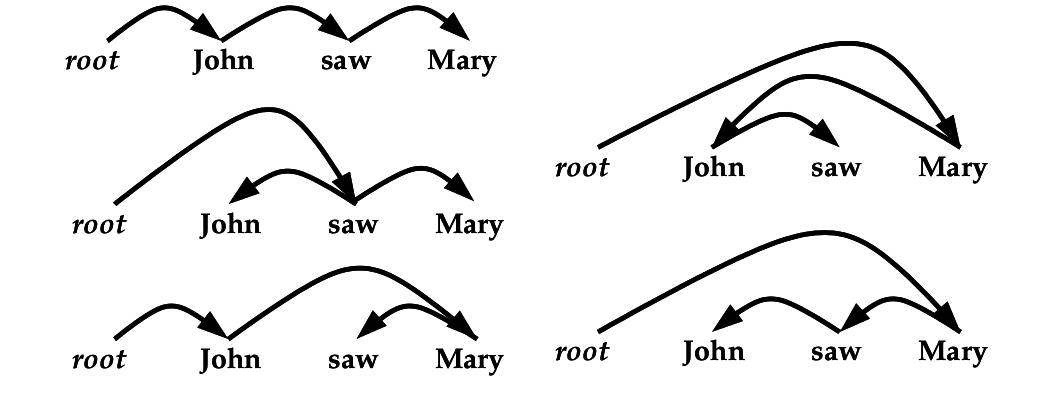
\includegraphics[width=90mm]{images/rsz_all_deps.jpg}
\label{overflow}
\end{figure}


Eisner’s parsing algorithm -- keep track of the counts of all possible parses.

A hypergraph -- efficient data structure -- calculating the probabilities of each one of these parses.
\end{frame}

\begin{frame}
\frametitle{Modified Eisner's parsing algorithm}

\begin{figure}
\centering
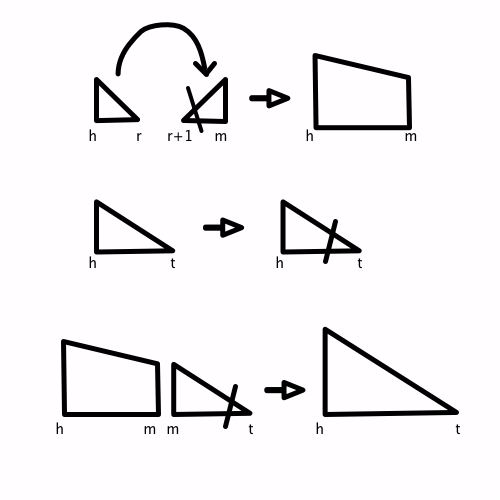
\includegraphics[width=90mm]{images/eisner_rules.jpg}
\caption{Eisner's algorithm rules}
\label{overflow}
\end{figure}

\end{frame}

\begin{frame}
\frametitle{Hypergraph}

A hypergraph  H = $(V, E)$, where $V$ is the set of vertices, $E$ is the set of hyperedges.

Hyperedge $e$ $\in$ $E$ of a weighted graph is a triple $e~=~(T(e), h(e), f(e))$, where $h(e)$ $\in$ $V$ is its head vertex and $T(e)$ $\in$ $V^*$ is an ordered list of tail vertices.

$f(e)$ is a weight function
\end{frame}

\begin{frame}

\begin{figure}
\centering
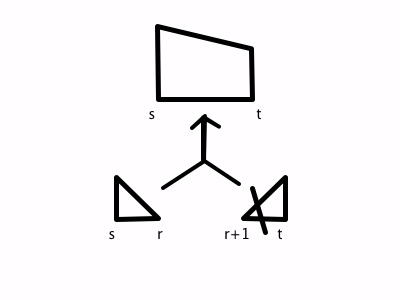
\includegraphics[width=90mm]{images/hypergraph_example.jpg}
\end{figure}

\end{frame}

\begin{frame}

\begin{figure}
\centering
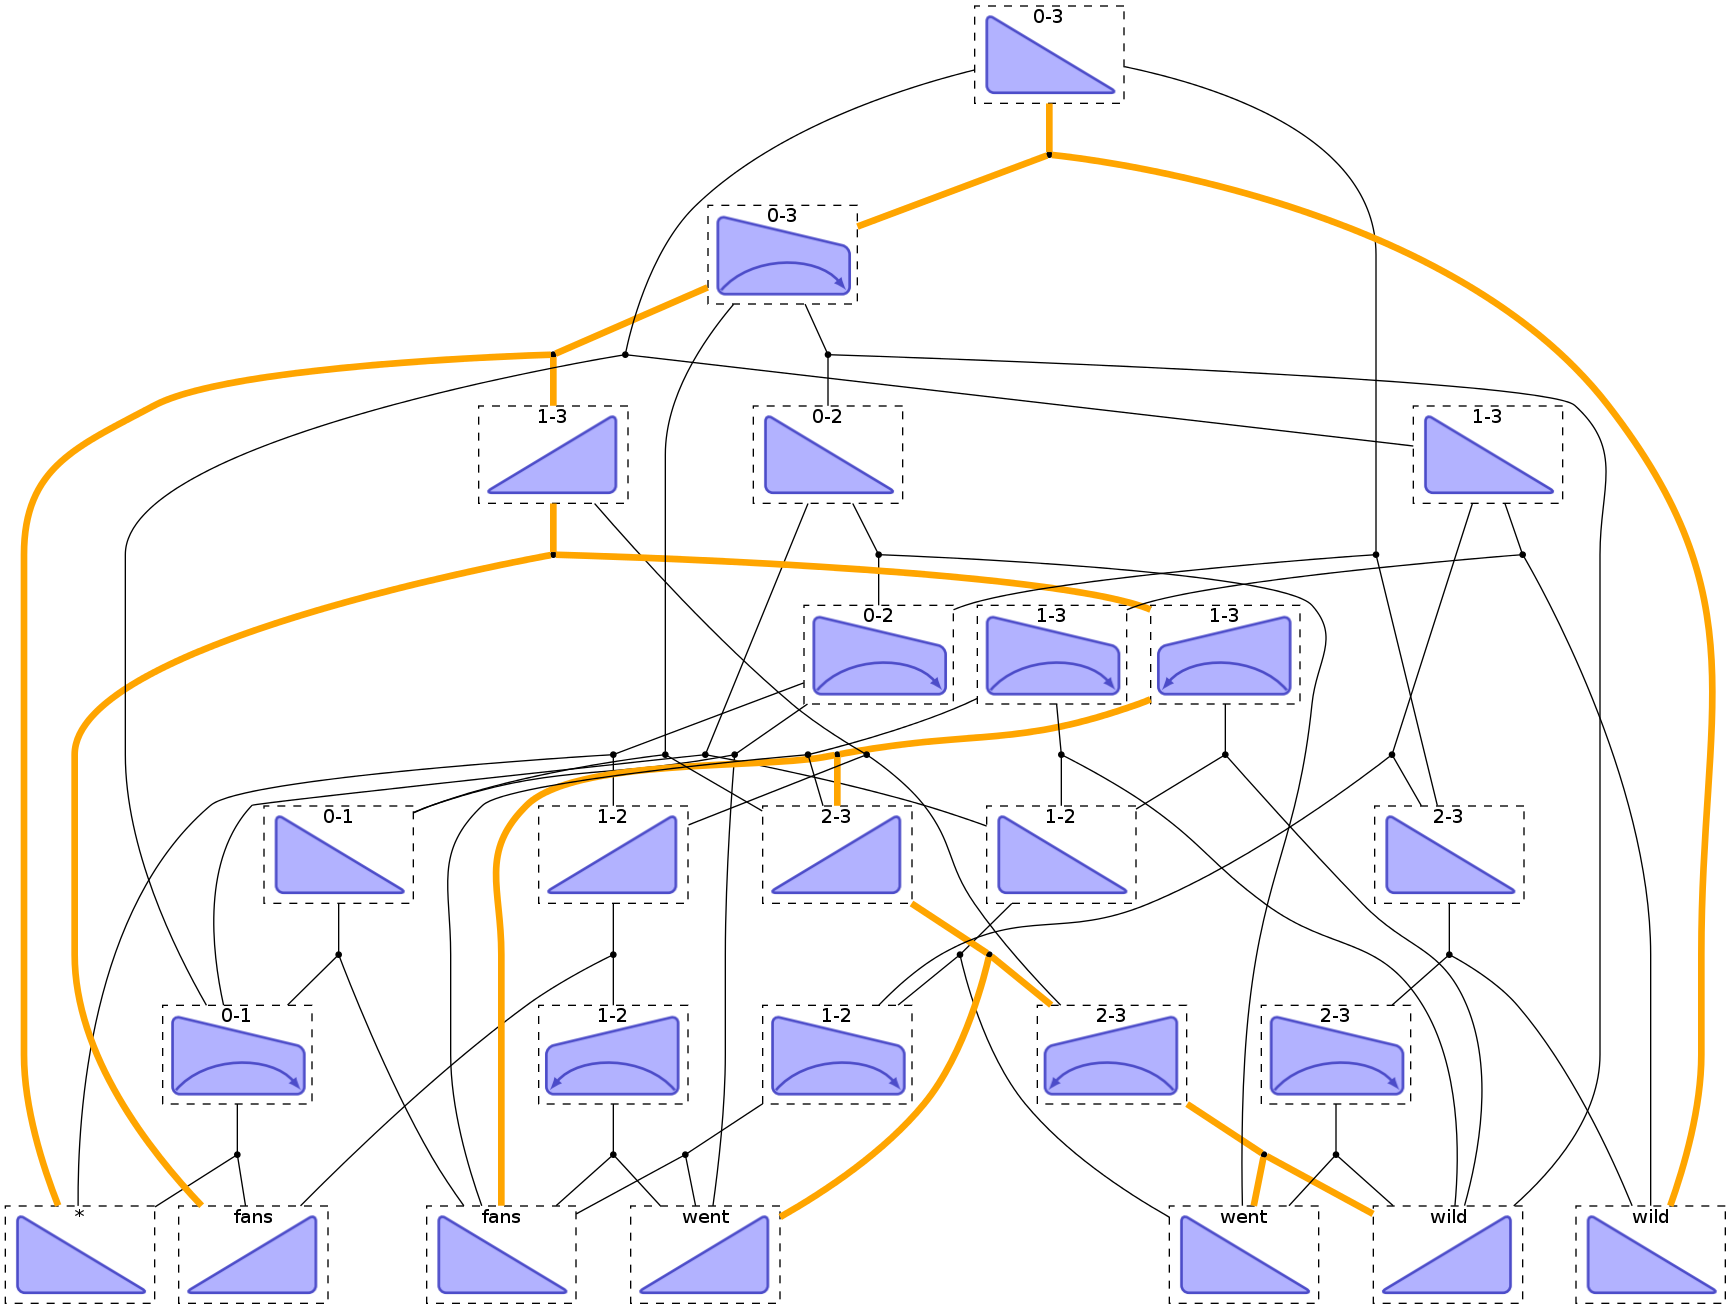
\includegraphics[width=90mm]{images/hypergraph.png}
\end{figure}

\end{frame}


\begin{frame}

\begin{algorithm}[H]
\caption{Compute Weights}
\begin{algorithmic}

\State Lets assume incomplete constituent as i.c and complete constituent stop as c.s

\If{edge.headNode $\in$ i.c}
   \State return depProb[edge.headWord, edge.modifierWord, edge.dir] $\times$ contProb[edge.headWord, edge.dir, edge.isAdj]
\ElsIf{edge.headNode $\in$ c.s}
   \State return stopProb[edge.headWord, edge.dir, edge.isAdj]
\Else
   \State return 1
\EndIf

\end{algorithmic}
\end{algorithm}

\end{frame}

\begin{frame}


\frametitle{Implementation}
\begin{itemize}

\item The insideOutside algorithm is run on the entire hypergraph.

\item  The inside probability of the root of the hypergraph gives the total probability of the sentence Z. 

\item The marginals of the nodes and the edges of the hypergraph are computed using the PyDecode library. 

\item counts = marginals / Z

\item The em algorithm is run 10 times for all the sentences

\end{itemize}
\end{frame}

\begin{frame}
\frametitle{Related work}


\begin{itemize}
\item (Smith and Eisner, 2005) used contrastive estimation together with DMV.
\item (Cohen et al., 2008) used logistic normal priors

\item (HeaddenIII et al., 2009) extended the valence and conditioned generating a new argument on whether it is adjacent or not. $P_{CHOOSE}(a|h, dir)$ in the above equation is thus substituted by $P_{CHOOSE}(a|h, dir, adj)$

\item (Spitkovsky et al., 2011) observed a strong connection between English punctuation and phrase boundaries, split sentences at punctuation marks and imposed parsing restrictions over their fragments.

\end{itemize}

\end{frame}

\begin{frame}

\frametitle{Initialization of DMV}
Consider a sentence with words $w_1$ $\ldots$ $w_n$ where $n$ is the number of words in the sentence.\\

(1) Each word has a uniform probability of becoming a ROOT.

   $$ P(ROOT) =  \frac{1}{n} $$

(2) The probability of dependency between two words is inversely proportional to the distance between them.

Linguistic intuition that shorter dependencies are preferable to longer

\end{frame}

\begin{frame}
\frametitle{Thousand random restarts}

\begin{algorithm}[H]

\caption{EM algorithm for a thousand random restarts}

\begin{algorithmic}

\For{iterations = 1 to 10}

   \For{sentence in corpus}

      \State Build hypergraph

      \For{multinomial in Multinomials}

         \State Update counts for sentence.  Estimation step

      \EndFor

   \EndFor

  \For{multinomial in Multinomials}

    \State Recompute the probabilities.  Maximization step

  \EndFor

\EndFor

\end{algorithmic}
\end{algorithm}

\end{frame}

\begin{frame}

\begin{figure}
\centering
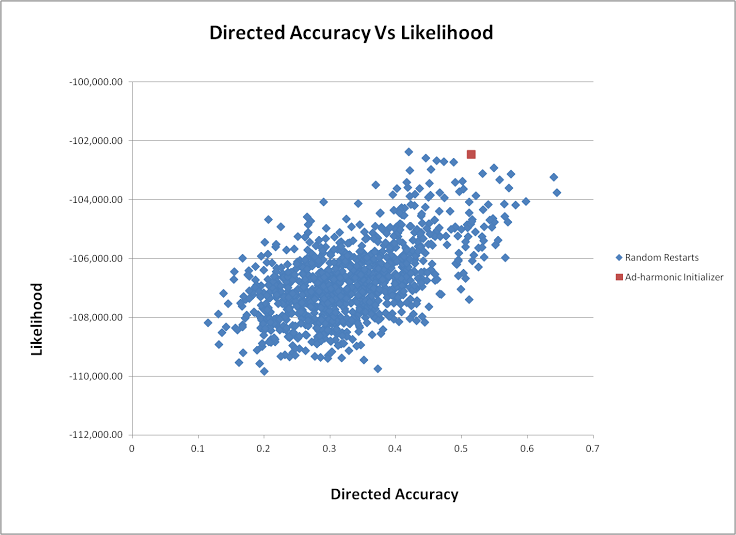
\includegraphics[width=90mm]{images/directed_accuracy.png}
\caption{Directed accuracy vs likelihood}
\label{overflow}
\end{figure}

\end{frame}


\begin{frame}

\begin{figure}
\centering
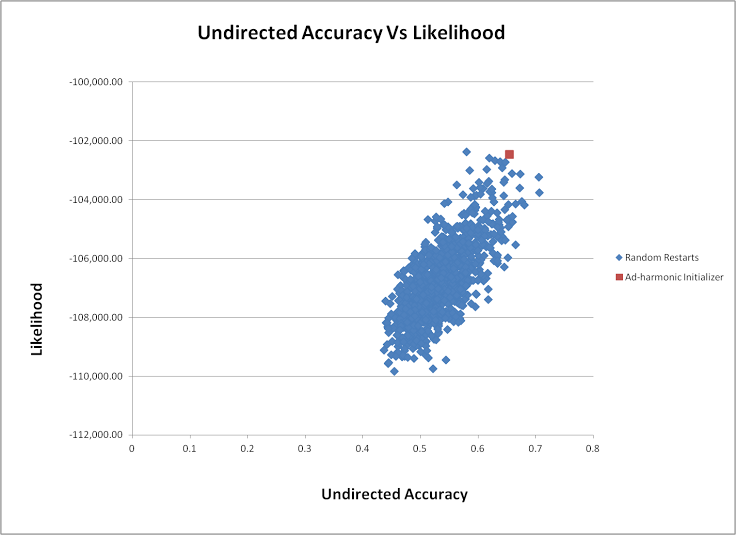
\includegraphics[width=90mm]{images/undirected_accuracy.png}
\caption{Undirected accuracy vs likelihood}
\label{overflow}
\end{figure}

\end{frame}

\begin{frame}
\begin{table}[htbp]
\begin{center}
\begin{tabular}{|l|c|r|}
\hline
\textbf{Characteristic} & \textbf{Ad-harmonic Initializer} & \textbf{Random Initializer}\\
\hline
Undirected accuracy &  65.5   &    70.56 (+5.06) \\
Directed accuracy &  51.5   &   55.59 (+4.09) \\
Likelihood &  -102,453.49   &  -102,375.79 (-77.7) \\
\hline
\end{tabular}
\end{center}
\caption{Comparing accuracies of Ad-harmonic and Random Initializer}
\end{table}

\end{frame}


\begin{frame}

\begin{figure}[!ht]
\centering
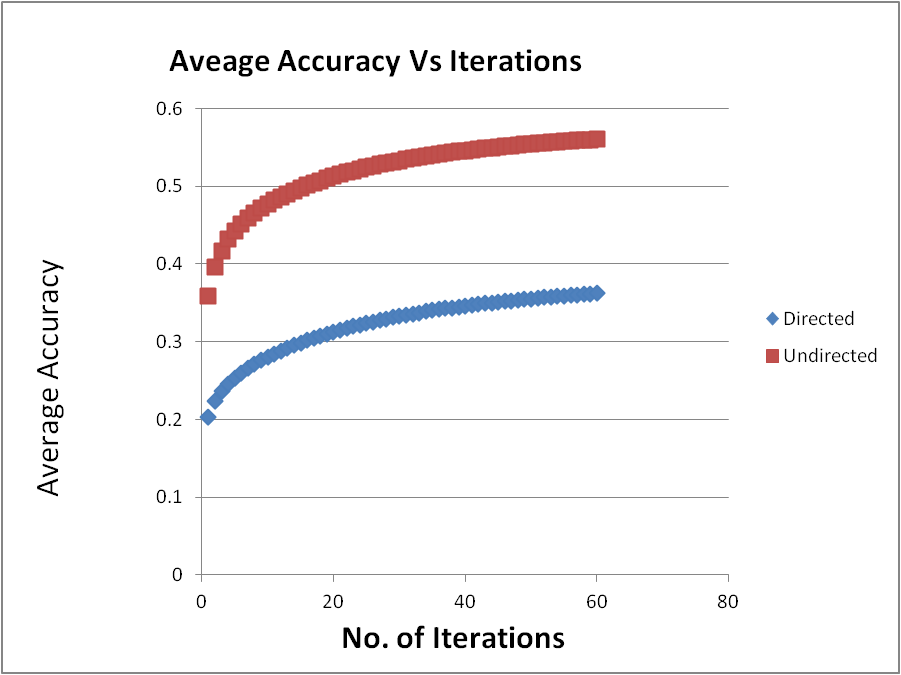
\includegraphics[width=90mm]{images/avg_accuracy.png}
\caption{Average accuracy per iteration}
\label{overflow}
\end{figure}

\end{frame}

\begin{frame}

\begin{figure}[!ht]
\centering
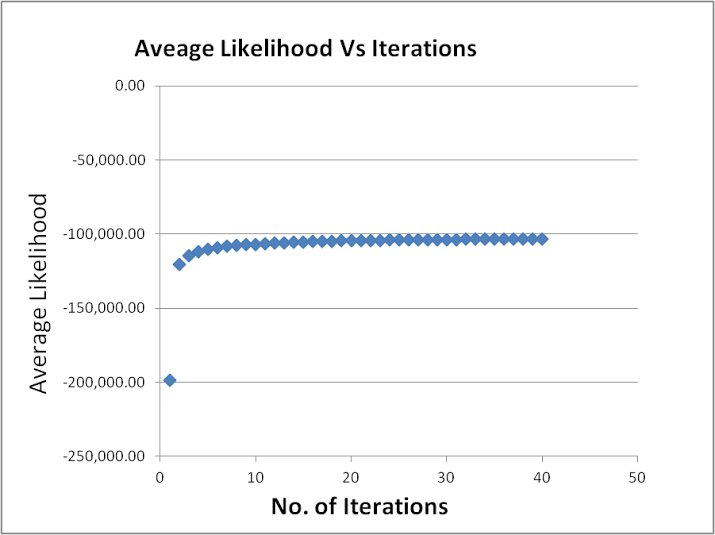
\includegraphics[width=90mm]{images/avg_likelihood.png}
\caption{Average likelihood per iteration}
\label{overflow}
\end{figure}

\end{frame}



\begin{frame}
\frametitle{Future Work}

\begin{itemize}
\item It takes 180 minutes to run EM for 60 iterations with 40 random restarts.

\item The time taken to build the model is directly proportional to the number of random restarts

\item To scale to a million random restarts, the time taken to build the model must be independent of the number of random restarts.

\end{itemize}
\end{frame}
\end{document}
